\documentclass{beamer}
\usetheme{Madrid}
\usepackage{amsmath, amssymb, graphicx}
\title[Constraint-Relaxation in PDE Inverse Problems]{An Analysis of Constraint-Relaxation in PDE-Based Inverse Problems}
\author{Tristan van Leeuwen and Yunan Yang}
\date{International Workshop on Operator Learning and its Applications}

\newcommand{\sU}{\mathsf{U}}
\newcommand{\sV}{\mathsf{V}}
\newcommand{\sC}{\mathsf{C}}

\newcommand{\mA}{\mathcal{A}}
\newcommand{\mP}{\mathcal{P}}
\newcommand{\mR}{\mathcal{R}}

\begin{document}

\begin{frame}
  \titlepage
\end{frame}

\begin{frame}{Motivation}
Inverse problems aim to estimate parameters in PDEs from observations.
\begin{itemize}
  \item Ubiquitous in science and engineering
  \item Typically formulated as PDE-constrained optimization
  \item Challenge: non-linearity, ill-posedness
\end{itemize}
\end{frame}

\begin{frame}{Examples}
Common applications:
\begin{itemize}
  \item Seismic imaging
  \item Medical imaging (e.g., MRI, EIT)
  \item Data assimilation in geosciences
\end{itemize}
%\includegraphics[width=0.8\textwidth]{example-placeholder}
\end{frame}

\begin{frame}{Outline}
\begin{enumerate}
  \item PDE-constrained optimization
  \item Main Results
  \item Case Studies
  \item Wrap-up
\end{enumerate}
\end{frame}

\begin{frame}{Classical Formulation}
Constrained optimization problem:
\begin{equation*}
\min_{c\in\sC} \frac{1}{2} \sum_{i,j} |\mP_i(u_j) - d_{ij}|^2 \quad \text{s.t. } \mA_c(u_j, \varphi) = \mP_j(\varphi) \,\,\, \forall \varphi \in \sU,
\end{equation*}
with
\begin{itemize}
  \item $\mA_c: \sU\times \sU \rightarrow \mathbb{C}$ a \emph{sesquilinear} form that denotes the PDE with coefficient $c$
  \item $\mP_i : \sU \rightarrow \mathbb{C}$ denotes the \emph{anti-linear} sampling operator, which we can also represent as $\mP_i = \langle p_i,\cdot \rangle_\sU$ with $p_i = \mR \mP_i$, with $\mR$ the \emph{linear} Riesz map
  \item $d_{ij} \in \mathbb{C}$ the measured data. 
\end{itemize}
\end{frame}

\begin{frame}{Relaxed Formulation}
We now relax the hard constraint by introducing auxiliary source terms $q_j$:
\begin{equation}
  \label{eq:relaxed}
\min_{c\in\sC, q\in\sU^n} \frac{1}{2} \sum_{i,j} |\mP_i(u_j) - d_{ij}|^2 + \frac{\rho}{2} \sum_j \|q_j\|_U^2
\end{equation}
Subject to:
\begin{equation*}
\mA_c(u_j, \varphi) = (\mP_j + \mR^{-1}q_j)(\varphi) \,\,\, \forall \varphi \in \sU,
\end{equation*}
\end{frame}

\begin{frame}{Rationale and challenges}
\begin{itemize}
  \item (+) The relaxation improves the optimization landscape and reduces sensitivity to initialization
  \item (-) Optimization over large space $\sC \times \sU^n$ (in stead of just $\sC$) makes it computationally much more demanding
\end{itemize}
\end{frame}

\begin{frame}{Representer Theorem}
\textbf{Lemma 1:} Minimizers $q_j$ of \eqref{eq:relaxed} are of the form
\begin{equation*}
q_j = \sum_{k=1}^n \overline{\alpha_{jk}} w_k
\end{equation*}
with $\overline{\mA_c(\varphi, w_k)} = \mP_k(\varphi),\, \forall \varphi\in\sU$ and $\alpha_{jk}\in\mathbb{C}$.
\end{frame}

\begin{frame}{Reduced Formulation}
\textbf{Lemma 2:}
The objective in \eqref{eq:relaxed} can be expressed in terms of $c$ alone as 
\begin{equation*}
J(c) = \frac{1}{2} \sum_{j=1}^n \|\mathbf{e}_j(c)\|_{(I + \rho^{-1} G(c))^{-1}}^2,
\end{equation*}
with
\begin{itemize}
  \item $e_{ij}(c) = d_{ij}-\mP_i(u_j)$ where $\mA_c(u_j,\varphi)\,\, \forall \varphi\in\sU$,
  \item $G(c)$ is Gram matrix from adjoint states:
\begin{equation*}
G_{ij}(c) = \langle w_i, w_j \rangle_U
\end{equation*}
\end{itemize}
\end{frame}

\begin{frame}{Limiting cases}
As $\rho\rightarrow\infty$ we recover the constrained formulation
\begin{equation*}
J_\infty(c) = \frac{1}{2} \sum_{j=1}^n \|\mathbf{e}_j(c)\|^2,
\end{equation*}
and for $\rho\rightarrow 0$ we get
\begin{equation*}
J_0(c) = \frac{\rho}{2} \sum_{j=1}^n \|\mathbf{e}_j\|_{G(c)^{-1}}^2
\end{equation*}
\end{frame}

\begin{frame}{Projected Residuals}
\textbf{Theorem 1: }
When the Riesz representers $\{p_i\}_{i=1}^n$ of the sources/receivers are orthonormal and the measurements are noiseless, the functional $J_\infty$ can be equivalently expressed in terms of an orthogonal projection of the solution-residual $u_i(c) - \check{u}_i \in \mathsf{U}$ on $\mathsf{P}_n = \text{span}\{p_i\}_{i=1}^n$ as
\[
J_{\infty}(c) = {\textstyle\frac{1}{2}}\sum_{j=1}^n\|\Pi_{\mathsf{P}_n}(u_j(c) - \check{u}_j)\|_{\mathsf{U}}^2,
\]
where $\Pi_{\mathsf{P}_n}:\sU\rightarrow\mathbb{C}^n$ is the orthogonal projection on $\mathsf{P}_n$, $u_j(c)$ is the weak solution corresponding to coefficient $c$, and $\check{u}_j$ is the true state corresponding to the true coefficient $\check{c}$.

\end{frame}

\begin{frame}{Projected Residuals}
\textbf{Theorem 2: }
For noiseless measurements, the functional $J_0(c)$ can be equivalently expressed in terms of an orthogonal projection of the PDE-residual $\mathcal{E}_j(c) = \mathcal{A}_c(\check{u}_j,\cdot) -  \mathcal{A}_{\check{c}}(\check{u}_j,\cdot) \in \mathsf{V}$, $j=1,\ldots,n$, on $\mathsf{W}_n = \text{span}\{w_j\}_{j=1}^n$ as
\[
J_0(c) = {\textstyle\frac{1}{2}}\sum_{j=1}^n \|\Pi_{\mathsf{W}_n}\mathcal{R}\mathcal{E}_j(c)\|_{\mathsf{U}}^2,
\]
with $\check{u}_j$ denoting the true state corresponding to the true coefficient $\check{c}$, and $w_j$ the adjoint solution for the current coefficient $c$.
\end{frame}


\begin{frame}{Projected Residuals}
This means that in the limit $\rho\rightarrow\infty$ we measure the error $c-\check{c}$ by looking at the residual
\[
u_j(c) - u_j(\check{c}),
\]
while for $\rho\rightarrow 0$ we consider
\[
\mathcal{A}_c(\check{u}_j,\cdot) -  \mathcal{A}_{\check{c}}(\check{u}_j,\cdot). 
\]
\end{frame}

\begin{frame}{Data-driven approach}
blabla
\end{frame}

\begin{frame}{Case Study: 1D Helmholtz ($n=2$)}
\begin{itemize}
  \item PDE: $-u_j'' - (k/c)^2 u_j = f_j, \quad u_j(0;k) = 0, u_j'(1;k)=\imath (k/c)u_j(1;k)$,
  \item Measure: $d_{ij} = \langle f_i, u_j\rangle_\sU$,
  \item Grammian can be obtained from measurements, allowing for a data-driven approach
\end{itemize}
\end{frame}

\begin{frame}{Case Study: 1D Helmholtz}

  \begin{center}
(conventional, \textcolor{blue}{variable metric}, \textcolor{orange}{data-driven metric})
  \end{center}
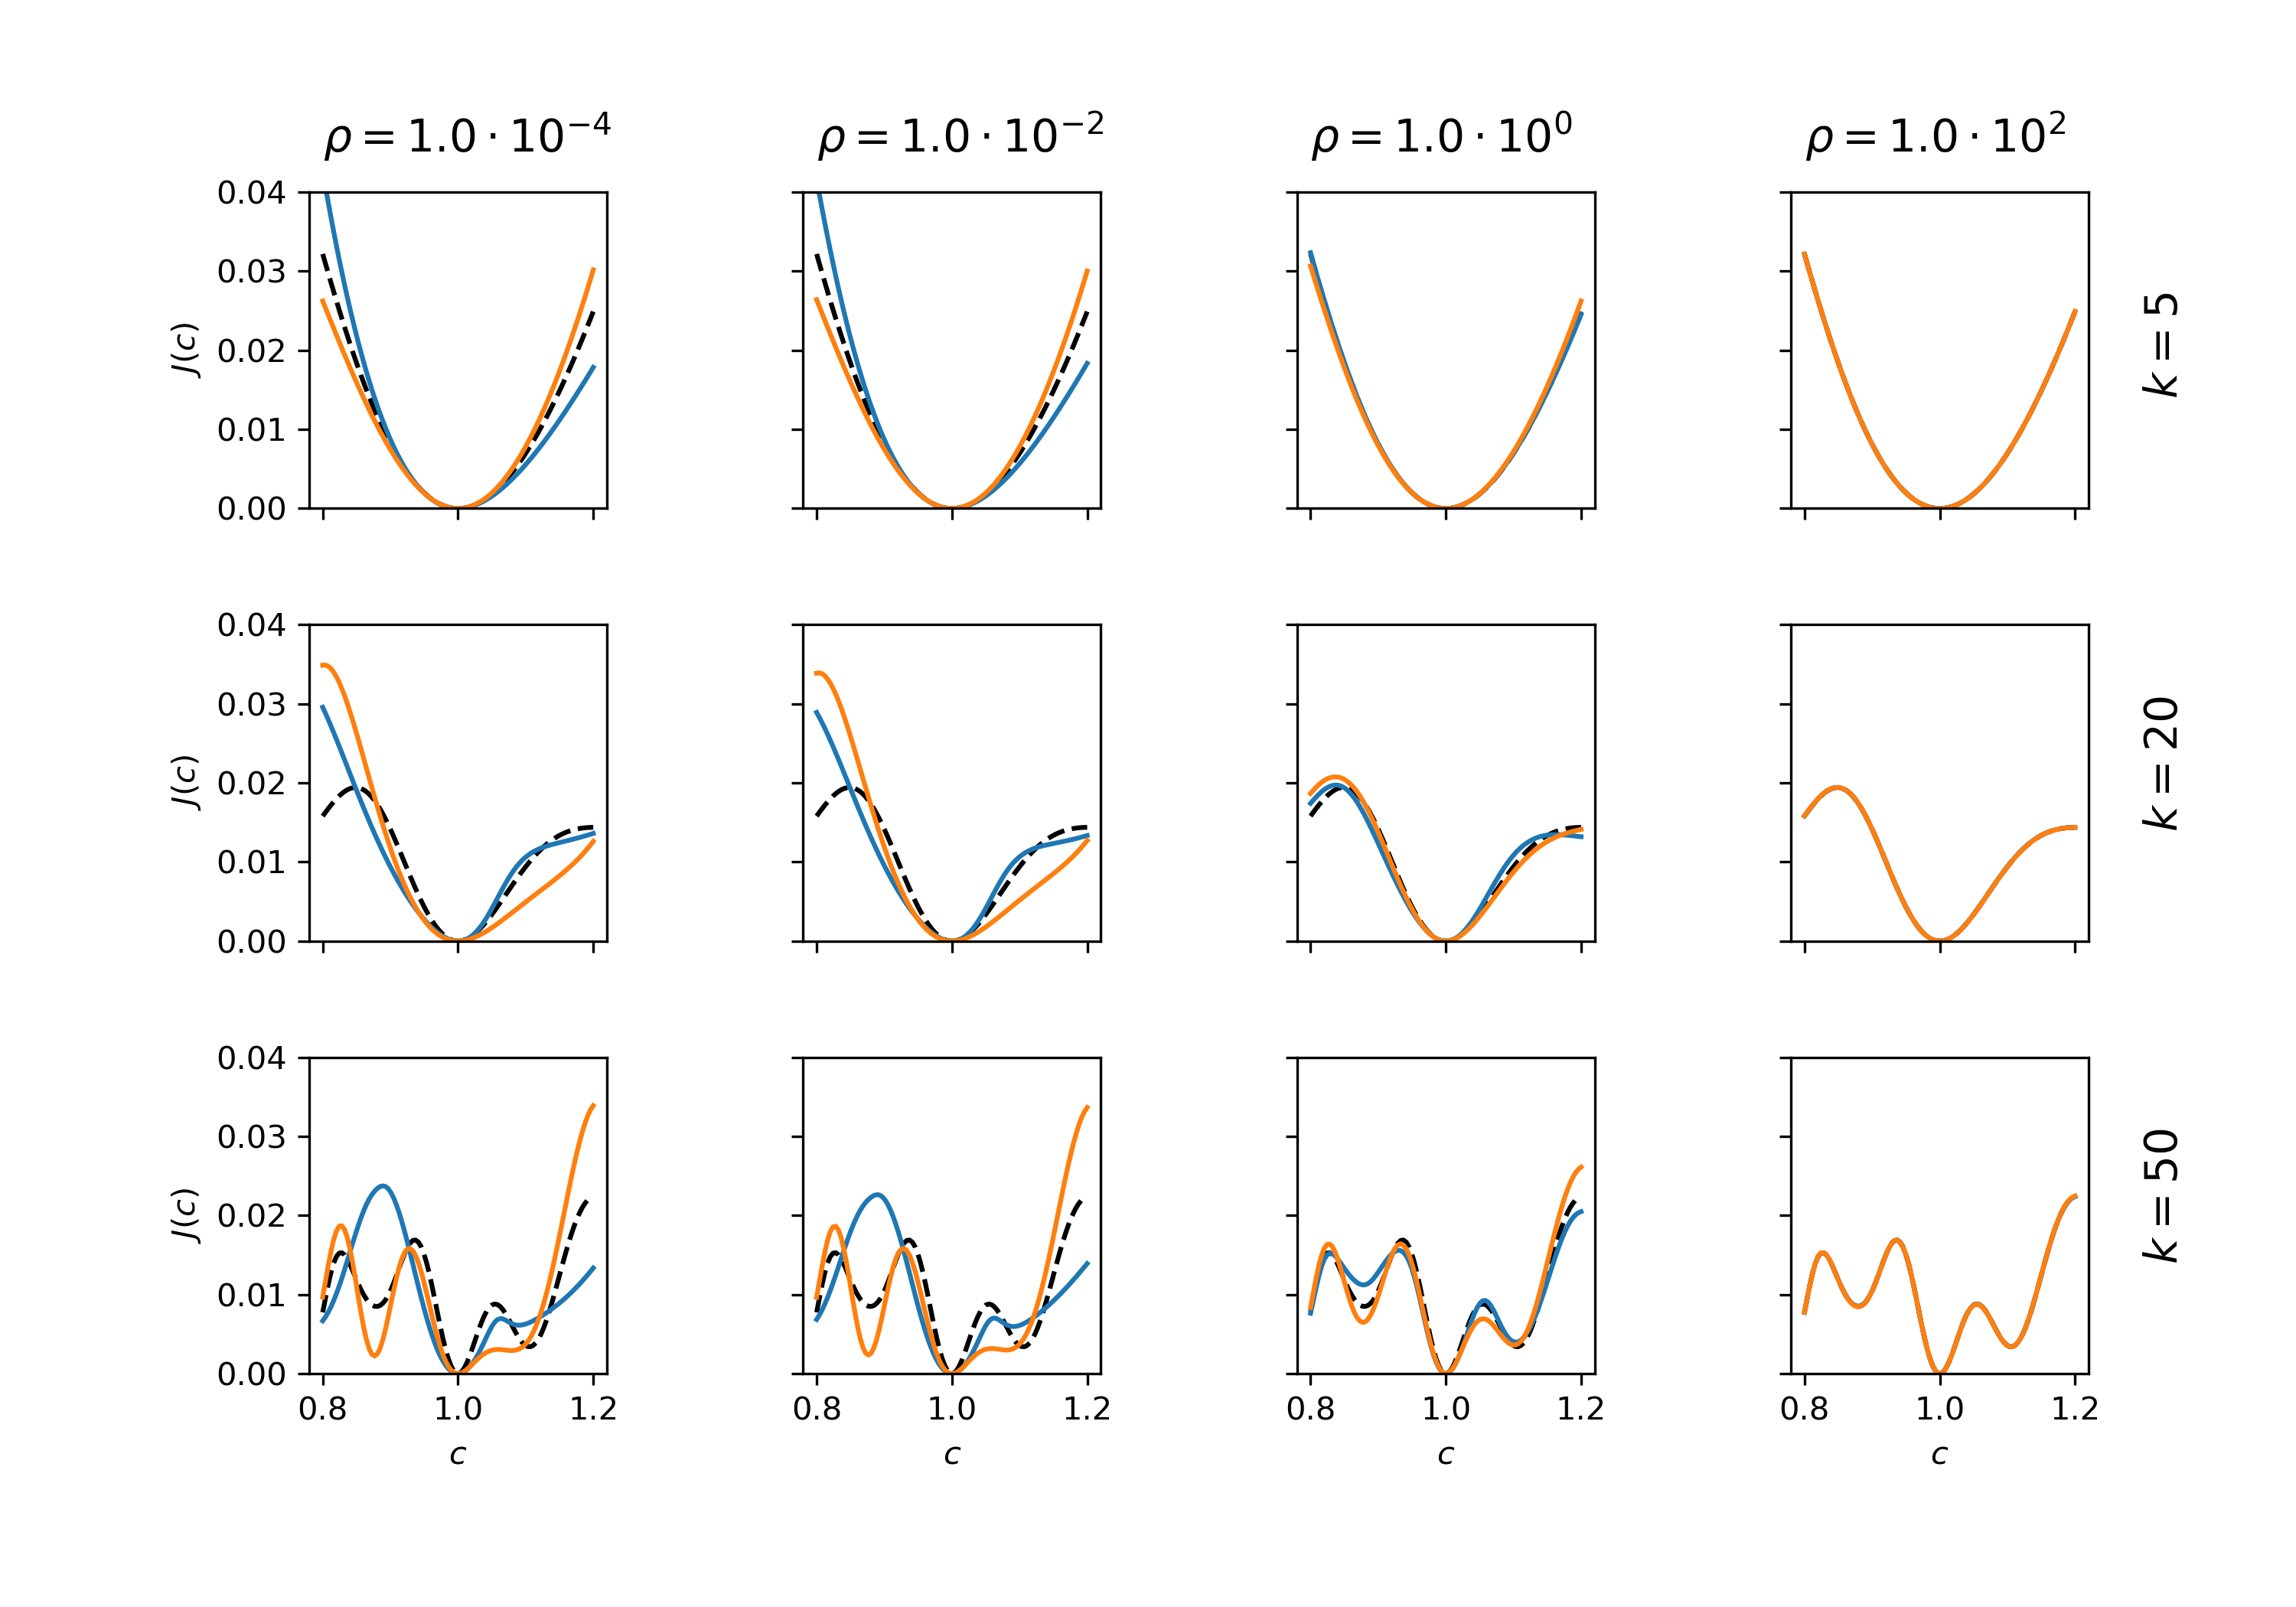
\includegraphics[width=0.9\textwidth]{../paper/figures/Helmholtz1D_2.png}
\end{frame}

\begin{frame}{Case Study: 2D Helmholtz}
\begin{itemize}
  \item Seismic inversion setup
  \item 124 sources/receivers
  \item Realistic starting models
\end{itemize}
\end{frame}

\begin{frame}{Case Study: 2D Helmholtz}
% \includegraphics[width=0.9\textwidth]{figure10-placeholder}
% \includegraphics[width=0.9\textwidth]{figure11-placeholder}
\end{frame}

\begin{frame}{Discussion}
\begin{itemize}
  \item Relaxation improves optimization landscape
  \item Bridges data-driven and PDE-based approaches
\end{itemize}
\end{frame}

\begin{frame}{Conclusion}
\begin{itemize}
  \item Presented unified framework for constraint-relaxation
  \item Shown reduced and limiting forms
  \item Case studies demonstrate advantages
\end{itemize}
\end{frame}

\begin{frame}{Acknowledgements}
\small
Thanks to collaborators, funding agencies, and the workshop organizers.
\end{frame}

\end{document}
